%\section{$S_{2}(P)$とコンパクト性}
\section{正規パターン集合のコンパクト性}

この節では,コンパクト性の定義を与え,$\sharp\Sigma \ge 2k-1$と仮定したとき,
$S_{2}(P)$は$\RPatL^{k}$における$L(P)$の特徴集合であることを示し,$\RPat^{k}$が包含に関してコンパクト性を持つことを示す.

\begin{dfn}
クラス$\mathcal{C} \subseteq \RPatplus$が\textbf{包含に関してコンパクト性を持つ}とは,
任意のパターン$p \in \RPat$と任意のパターン集合$Q \in \mathcal{C}$に対して,
$L(p) \subseteq L(Q)$ならば,ある$q \in Q$が存在して$L(p) \subseteq L(q)$であるときをいう.
\end{dfn}
%\begin{comment}
同様にして,クラス$\mathcal{C} \in \Patplus$が包含に関してコンパクト性を持つことが定義できる.
また,クラス$\mathcal{C} \in \RPatplus$が包含に関してコンパクト性を持つとき,補題\ref{補題1}より,任意の$P, Q \in \mathcal{C}$に対して,$P \sqsubseteq Q$ならばその時に限り$L(P) \subseteq L(Q)$であることが示せる.

\begin{lem}[Sato et al.\cite{Sato1}]\label{変数2つ}
$\sharp \Sigma \ge 3$とし,$p,~q$を正規パターンとする.
正規パターンの有限集合$D$が,次の{\rm (i), (ii)}のいずれかで表されるとき,任意の$r \in D$に対して$p \{ x := r \} \preceq q$ならば,$p \{ x := xy \} \preceq q$である.
ただし,$a \ne b$とする.
\[
\begin{tabular}{ll}
$(\mathrm{i})$ $\{ ay, by \}$,
$(\mathrm{ii})$ $\{ ya, yb \}$.
\end{tabular}
\]
\end{lem}
\begin{proof}
$p$に変数記号が含まれない場合は自明である.
したがって,正規パターン$p$には変数記号が現れるとし,その変数記号を$x$とする.
このとき,正規パターン$p_{1},p_{2}$が存在し,$p=p_{1}xp_{2}$と表すことができる.$p \{ x := xy \} \not \preceq q$と仮定して,矛盾を導く.
\smallskip

\noindent
\textbf{(i)} $D=\{ ay, by \} \ (a \ne b)$であるとする.
$p \{ x := xy \} \not \preceq q$のとき,$p_{1}ayp_{2}\preceq q$かつ$p_{1}byp_{2}\preceq q$であることから,正規パターン$q_{1},q_{2}$と変数記号$y_{1},y_{2}$,さらに定数記号列$w$が存在して,$q=q_{1}ay_{1}wby_{2}q_{2}$または$q=q_{1}by_{1}way_{2}q_{2}$と表すことができる.$q=q_{1}ay_{1}wby_{2}q_{2}$と表されるとき,次の(1), (2), (1'), (2')がすべて成り立つ.
\[
\begin{tabular}{llll}
(1) & $p_{1} \preceq q_{1}$ & (1') & \begin{minipage}[t]{3.5cm}$p_{2} \preceq wby_{2}q_{2}$または\\$p_{2} \preceq y^{\prime}wby_{2}q_{2}$\end{minipage} \\
(2) & $p_{1} \preceq q_{1}ay_{1}w$ & (2') & $p_{2} \preceq q_{2}$または$p_{2} \preceq y^{\prime\prime}q_{2}$
\end{tabular}
\]

(2)より,正規パターン$p_{1}^{\prime},p_{1}^{\prime\prime}$が存在して,
$p_{1}=p_{1}^{\prime}p_{1}^{\prime\prime}$,$p_{1}^{\prime} \preceq q_{1}a$かつ$p_{1}^{\prime\prime} \preceq y_{1}w$
が成り立つ.
したがって,
$p=p_{1}xp_{2}=p_{1}^{\prime}p_{1}^{\prime\prime}xp_{2}$であるから,(1')が$p_{2} \preceq wby_{2}q_{2}$のとき,
$p\preceq q_{1}ap_{1}^{\prime\prime}xwby_{2}q_{2}=q \{ y_{1} := p_{1}^{\prime\prime}x \}$となる.また,(1')が$p_2\preceq y'wby_{2}q_{2}$のとき,$p\preceq q_{1}ap_{1}^{\prime\prime}xy'wby_{2}q_{2}=q \{ y_{1} := p_{1}^{\prime\prime}xy' \}$となる.
よって,$p \preceq q$が成り立ち,
仮定$p \{ x := xy \} \not\preceq q$に矛盾する.
\smallskip

\noindent
\textbf{(ii)} $D=\{ ya, yb \} \ (a \ne b)$のときは,記号列$p$と$q$を逆順にすることにより,\textbf{(i)}の場合と同様に, 仮定$p \{ x := xy \} \not\preceq q$に矛盾することを証明できる.
\end{proof}

\begin{lem}\label{補題14}
$\sharp \Sigma \ge 4$とし,$p, q$を正規パターンとする.
正規パターンの有限集合$D= \{ a_{1}b_{1}, a_{2}b_{2}, a_{3}b_{3}, a_{4}b_{4} \}$ $(i \ne j $に対して,$a_{i} \ne a_{j}$かつ$b_{i} \ne b_{j})$で表されるとき,任意の$r \in D$に対して$p \{ x := r \} \preceq q$ならば,$p \{ x := xy \} \preceq q$である.
\end{lem}
\begin{proof}
$p$に変数記号が含まれない場合は自明である.
したがって,正規パターン$p$には変数記号が現れるとし,その変数記号を$x$とする.
このとき,正規パターン$p_{1},p_{2}$が存在し,$p=p_{1}xp_{2}$と表すことができる.
$p \{ x := xy \} \not \preceq q$と仮定して,矛盾を導く.

$D=\{ a_{1}b_{1}, a_{2}b_{2}, a_{3}b_{3}, a_{4}b_{4} \}$ $(i \ne j$に対して,$a_{i} \ne a_{j}$かつ$b_{i} \ne b_{j})$であるとする.
任意の$r \in D$に対して$p \{ x := r \} \preceq q$であることから,
正規パターン$q$には,$a_{1}b_{1}, a_{2}b_{2}, a_{3}b_{3}, a_{4}b_{4}$に対応する長さ2の記号列が存在する.
その4つの記号列は一部を重複して現れることがあることに注意する.
$D$の4つの記号列に対応する$q$の記号列の現れ方には次の15通り存在する.
\[
\begin{tabular}{ll}
(a) $a_{1}b_{1}, a_{2}b_{2}, a_{3}b_{3}, a_{4}b_{4}$    & (i) $a_{1}b_{1}, y_{1}b_{2}, a_{3}y_{2}, a_{4}y_{3}$ \\
(b) $a_{1}b_{1}, a_{2}b_{2}, a_{3}b_{3}, a_{4}y_{1}$        & (j) $a_{1}b_{1}, a_{2}y_{1}, a_{3}y_{2}, a_{4}y_{3}$ \\
(c) $a_{1}b_{1}, a_{2}b_{2}, a_{3}b_{3}, y_{1}b_{4}$        & (k) $y_{1}b_{1}, y_{2}b_{2}, y_{3}b_{3}, y_{4}b_{4}$ \\
(d) $a_{1}b_{1}, a_{2}b_{2}, a_{3}y_{1}, y_{2}b_{4}$            & (l) $y_{1}b_{1}, y_{2}b_{2}, y_{3}b_{3}, a_{4}y_{4}$ \\
(e) $a_{1}b_{1}, a_{2}b_{2}, y_{1}b_{3}, y_{2}b_{4}$            & (m) $y_{1}b_{1}, y_{2}b_{2}, a_{3}y_{3}, a_{4}y_{4}$ \\
(f) $a_{1}b_{1}, a_{2}b_{2}, a_{3}y_{1}, a_{4}y_{2}$            & (n) $y_{1}b_{1}, a_{2}y_{2}, a_{3}y_{3}, a_{4}y_{4}$ \\
(g) $a_{1}b_{1}, y_{1}b_{2}, y_{2}b_{3}, y_{3}b_{4}$                & (o) $a_{1}y_{1}, a_{2}y_{2}, a_{3}y_{3}, a_{4}y_{4}$ \\
(h) $a_{1}b_{1}, y_{1}b_{2}, y_{2}b_{3}, a_{4}y_{3}$  & ($y_{1},y_{2},y_{3},y_{4}$は変数記号)
\end{tabular}
\]

上記\textbf{(e)--(o)}の11通りの記号列を含む正規パターン$q$は,
補題\ref{変数2つ}(i)または(ii)に対応する記号列が現れる.
その場合の証明より仮定$p \{ x := xy \} \not\preceq q$に矛盾する.
したがって,(a)--(d)の4通りついて矛盾を導く.

(a), (b), (c)は,$q$に$a_{1}b_{1}, a_{2}b_{2}, a_{3}b_{3}, a_{4}b_{4}$が現れる場合,(d)は, $q$に$a_{1}b_{1}, a_{2}b_{2}, a_{3}y_{1}, y_{2}b_{4}$が現れる場合において,矛盾を導く証明が考えられる.
しかし,(a), (b), (c)は,$q$に$a_{1}b_{1}, a_{2}b_{2}, a_{3}b_{3}$が現れる場合,(d)は, $q$に$a_{1}b_{1}, a_{2}b_{2}, a_{3}y_{1}$が現れる場合と$q$に$a_{1}b_{1}, a_{2}b_{2}, y_{2}b_{4}$が現れる場合において,矛盾を導くことで,証明できる.
よって,本論文では,$q$に$a_{1}b_{1}, a_{2}b_{2}, a_{3}b_{3}$が現れる場合と$q$に$a_{1}b_{1}, a_{2}b_{2}, a_{3}y$ $(y=y_{1})$が現れる場合を証明する.
$q$に$a_{1}b_{1}, a_{2}b_{2}, y_{2}b_{4}$が現れる場合は,記号列$p$と$q$を逆順にすることにより,$q$に$a_{1}b_{1}, a_{2}b_{2}, a_{3}y$が現れる場合の証明から導かれる.
\smallskip

\noindent
\textbf{(abc)} $q$に$a_{1}b_{1}, a_{2}b_{2}, a_{3}b_{3}$が現れる場合,

%\begin{figure}[H]
\begin{figure}
\centering
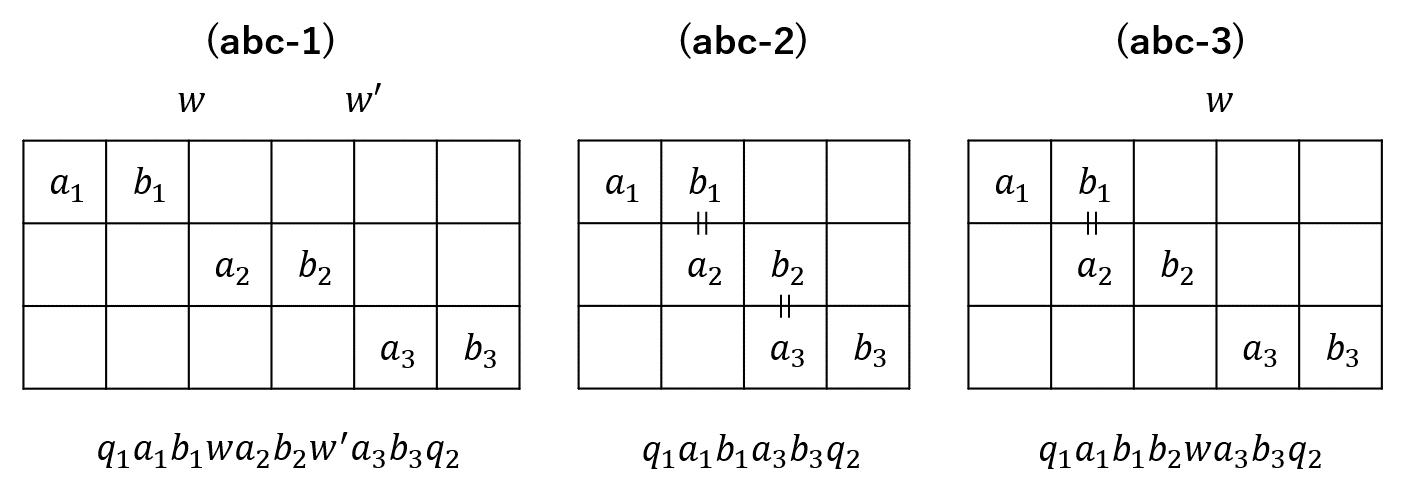
\includegraphics[width=\linewidth]{figs/Cases-abc.png}
\vspace{-1cm}
\caption{(abc)の場合分け}
\label{abc組み合わせ}
\end{figure}

図\ref{abc組み合わせ}のように,3つの記号列が重複する場合があるので,次の3つの場合に分けて証明する.
\[
\begin{tabular}{ll}
$\textbf{(abc-1)}$ $q=q_{1}a_{1}b_{1}wa_{2}b_{2}w^{\prime}a_{3}b_{3}q_{2}$,\\
$\textbf{(abc-2)}$ $q=q_{1}a_{1}b_{1}a_{3}b_{3}q_{2}$ ($b_{1}=a_{2}$かつ$a_{3}=b_{2}$),\\
$\textbf{(abc-3)}$ $q=q_{1}a_{1}b_{1}b_{2}wa_{3}b_{3}q_{2}$ ($b_{1}=a_{2}$).
\end{tabular}
\]

\textbf{(abc-1)} $q=q_{1}a_{1}b_{1}wa_{2}b_{2}w^{\prime}a_{3}b_{3}q_{2}$とする.これに対して,次の式が成り立っているものとする.
\begin{align*}
(1)~& p_{1} \preceq q_{1} & (\text{1'})~& p_{2} \preceq wa_{2}b_{2}w^{\prime}a_{3}b_{3}q_{2} \\
(2)~& p_{1} \preceq q_{1}a_{1}b_{1}w & (\text{2'})~& p_{2} \preceq w^{\prime}a_{3}b_{3}q_{2} \\
(3)~& p_{1} \preceq q_{1}a_{1}b_{1}wa_{2}b_{2}w^{\prime} & (\text{3'})~& p_{2} \preceq q_{2}
\end{align*}

$|w|=|w^{\prime}|$のとき,(2)と(3)より,$p_{1}$の接尾辞は$a_{1}b_{1}wa_{2}b_{2}w^{\prime}$かつ$a_{1}b_{1}w$であるので,$a_{1}b_{1}w=a_{2}b_{2}w^{\prime}$となる.よって,$a_{1}b_{1}=a_{2}b_{2}$となり,$a_{1} \ne a_{2}$かつ$b_{1} \ne b_{2}$であることに矛盾する.

$|w|+1=|w^{\prime}|$のとき,(1')と(2')より,$p_{2}$の接頭辞は$wa_{2}b_{2}w^{\prime}a_{3}b_{3}$かつ$w^{\prime}a_{3}b_{3}$である.
$w^{\prime}=ww_{1}$とおくと,$w^{\prime}a_{3}b_{3}=ww_{1}a_{3}b_{3}$となる.
したがって,$wa_{2}b_{2}=ww_{1}a_{3}$より$b_{2}=a_{3}$となる.
(2)と(3)より,$p_{1}$の接尾辞は$a_{1}b_{1}wa_{2}b_{2}w^{\prime}, a_{1}b_{1}w$である.$w^{\prime}=w_{2}w$とおくと,$a_{1}b_{1}wa_{2}b_{2}w^{\prime}=a_{1}b_{1}wa_{2}b_{2}w_{2}w$となる.
したがって,$b_{2}w_{2}w=a_{1}b_{1}w$より,$b_{2}=a_{1}$となる.
$b_{2}=a_{3}$より,$a_{3}=a_{1}$となり,$a_{3} \ne a_{1}$であることに矛盾する.

$|w|+1 < |w^{\prime}|$のとき,(2)と(3)より,$p_{1}$の接尾辞は$a_{1}b_{1}wa_{2}b_{2}w^{\prime}$かつ$a_{1}b_{1}w$である.
$w^{\prime}=w_{1}w$とおくと,$a_{1}b_{1}wa_{2}b_{2}w^{\prime}=a_{1}b_{1}wa_{2}b_{2}w_{1}w$となる.
$|w_{1}| \ge 2$であるため,$w_{1}$の接尾辞は$a_{2}b_{2}$となる.
($1'$)と($2'$)より,$p_{2}$の接頭辞は$wa_{2}b_{2}w^{\prime}a_{3}b_{3}$かつ$w^{\prime}a_{3}b_{3}$である.
$w^{\prime}=ww_{2}$とおくと,$w^{\prime}a_{3}b_{3}=ww_{2}a_{3}b_{3}$となり,$w^{\prime}=w_{1}w$とおくと,$wa_{2}b_{2}w^{\prime}a_{3}b_{3}=wa_{2}b_{2}w_{1}wa_{3}b_{3}$となる.
$|ww_{2}a_{3}b_{3}|=|wa_{2}b_{2}w_{1}|$より,$w_{1}$の接尾辞は$a_{3}b_{3}$となる.
よって,$w_{1}$の接尾辞は$a_{2}b_{2}=a_{3}b_{3}$となり,$a_{2} \ne a_{3}$かつ$b_{2} \ne b_{3}$であることに矛盾する.
\smallskip

\textbf{(abc-2)} $q=q_{1}a_{1}b_{1}a_{3}b_{3}q_{2}$ ($b_{1}=a_{2}$かつ$a_{3}=b_{2}$)とする.
これに対して,次の式が成り立っているものとする.
\begin{align*}
(1)~& p_{1} \preceq q_{1} & (\text{1'})~& p_{2} \preceq a_{3}b_{3}q_{2} \\
(2)~& p_{1} \preceq q_{1}a_{1} & (\text{2'})~& p_{2} \preceq b_{3}q_{2} \\
(3)~& p_{1} \preceq q_{1}a_{1}b_{1} & (\text{3'})~& p_{2} \preceq q_{2}
\end{align*}

(2)と(3)より,$p_{1}$の接尾辞は$a_{1}b_{1}$かつ$a_{1}$であり,$b_{1}=a_{1}$となる.$b_{1}=a_{2}$より,$a_{1}=a_{2}$であるため, $a_{1} \ne a_{2}$であることに矛盾する.
\smallskip

\textbf{(abc-3)} $q=q_{1}a_{1}b_{1}b_{2}wa_{3}b_{3}q_{2}$ ($b_{1}=a_{2}$)とする.これに対して,次の式が成り立っているものとする.
\begin{align*}
(1)~& p_{1} \preceq q_{1} & (\text{1'})~& p_{2} \preceq b_{2}wa_{3}b_{3}q_{2} \\
(2)~& p_{1} \preceq q_{1}a_{1} & (\text{2'})~& p_{2} \preceq wa_{3}b_{3}q_{2} \\
(3)~& p_{1} \preceq q_{1}a_{1}b_{1}b_{2}w & (\text{3'})~& p_{2} \preceq q_{2}
\end{align*}

$w=\varepsilon$のとき,(2)と(3)より,$p_{1}$の接尾辞は$a_{1}$かつ$a_{1}b_{1}b_{2}$であり,(1')と(2')より,$p_{2}$の接頭辞は$b_{2}a_{3}b_{3}$かつ$a_{3}b_{3}$である.
$b_{2}=a_{1}$と$b_{2}a_{3}=a_{3}b_{3}$より,$a_{1}=a_{3}$となり,$a_{1} \ne a_{3}$であることに矛盾する.

$|w| \ge 1$のとき,(2)と(3)より,$p_{1}$の接尾辞は$a_{1}$かつ$a_{1}b_{1}b_{2}w$である.
よって,$w$の最後の記号は$a_{1}$となる.
(1')と(2')より,$p_{2}$の接頭辞は$b_{2}wa_{3}b_{3}$かつ$wa_{3}b_{3}$となる.
よって,$w$の最後の記号は$a_{3}$となる.
したがって,$w$の最後の記号は$a_{1}=a_{3}$となり,$a_{1} \ne a_{3}$であることに矛盾する.
\smallskip

\textbf{(d)} $q$に$a_{1}b_{1}, a_{2}b_{2}, a_{3}y$が現れる場合,記号列$A,B,C$に対して,$\{ A, B, C \} = \{ a_{1}b_{1}, a_{2}b_{2}, a_{3}y \}$とおき,$q=q_{1}AwBw^{\prime}Cq_{2}$とする.
これに対して,次の式が成り立っているものとする.
\begin{align*}
(1)~& p_{1} \preceq q_{1} & (\text{1'})~& p_{2} \preceq wBw^{\prime}Cq_{2} \\
(2)~& p_{1} \preceq q_{1}Aw & (\text{2'})~& p_{2} \preceq w^{\prime}Cq_{2} \\
(3)~& p_{1} \preceq q_{1}AwBw^{\prime} & (\text{3'})~& p_{2} \preceq q_{2}
\end{align*}

$|w|=|w^{\prime}|$のとき,(2)と(3)より,$p_{1}$の接尾辞は$Aw$かつ$AwBw^{\prime}$である.
よって,$Aw=Bw^{\prime}$となり,$A \ne B$であることに矛盾する.

$|w| \ne |w^{\prime}|$とする.
$A=a_{3}y$とすると,$B=a_{1}b_{1}$,$C=a_{2}b_{2}$としてよいので,(2)は$p_{1} \preceq q_{1}a_{3}yw$となる.
したがって,正規パターン$p_{1}', p_{1}''$が存在して,$p_{1}=p_{1}'p_{1}''$,$p_{1}^{\prime} \preceq q_{1}a_{3}$かつ$p_{1}^{\prime\prime} \preceq yw$となる.
これらと(1')より,$p=p_{1}xp_{2}=p_{1}^{\prime}p_{1}^{\prime\prime}xp_{2}\preceq q_{1}a_{3}p_{1}^{\prime\prime}xwa_{1}b_{1}w^{\prime}a_{2}b_{2}q_{2}=q \{ y := p_{1}^{\prime\prime}x \}$となり,$p=q \theta$となる.
これは仮定に矛盾する.
$B=a_{3}y$とすると,$A=a_{1}b_{1}$,$C=a_{2}b_{2}$としてよいので,(3)は$p_{1} \preceq q_{1}a_{1}b_{1}wa_{3}yw^{\prime}$となり,(1')は$p_{2} \preceq wa_{3}yw^{\prime}a_{2}b_{2}q_{2}$である.$q_{1}^{\prime}=q_{1}a_{1}b_{1}$,$q_{2}^{\prime}=wa_{3}yw^{\prime}$,$q_{3}^{\prime}=a_{2}b_{2}q_{2}$とおくと, (3)~$p_{1} \preceq q_{1}^{\prime}q_{2}^{\prime}, (1')~p_{2} \preceq q_{2}^{\prime}q_{3}^{\prime}, q_{2}^{\prime}$は変数記号が含まれる.
補題\ref{補題9}より,$p \preceq q$となり,$p \{ x := xy \} \preceq q$である.
これは仮定に矛盾する.

以上より,$A$または$B$が$a_{3}y$の場合,仮定に矛盾するため,$C=a_{3}y$となる.

%\begin{figure}[H]
\begin{figure}
\centering
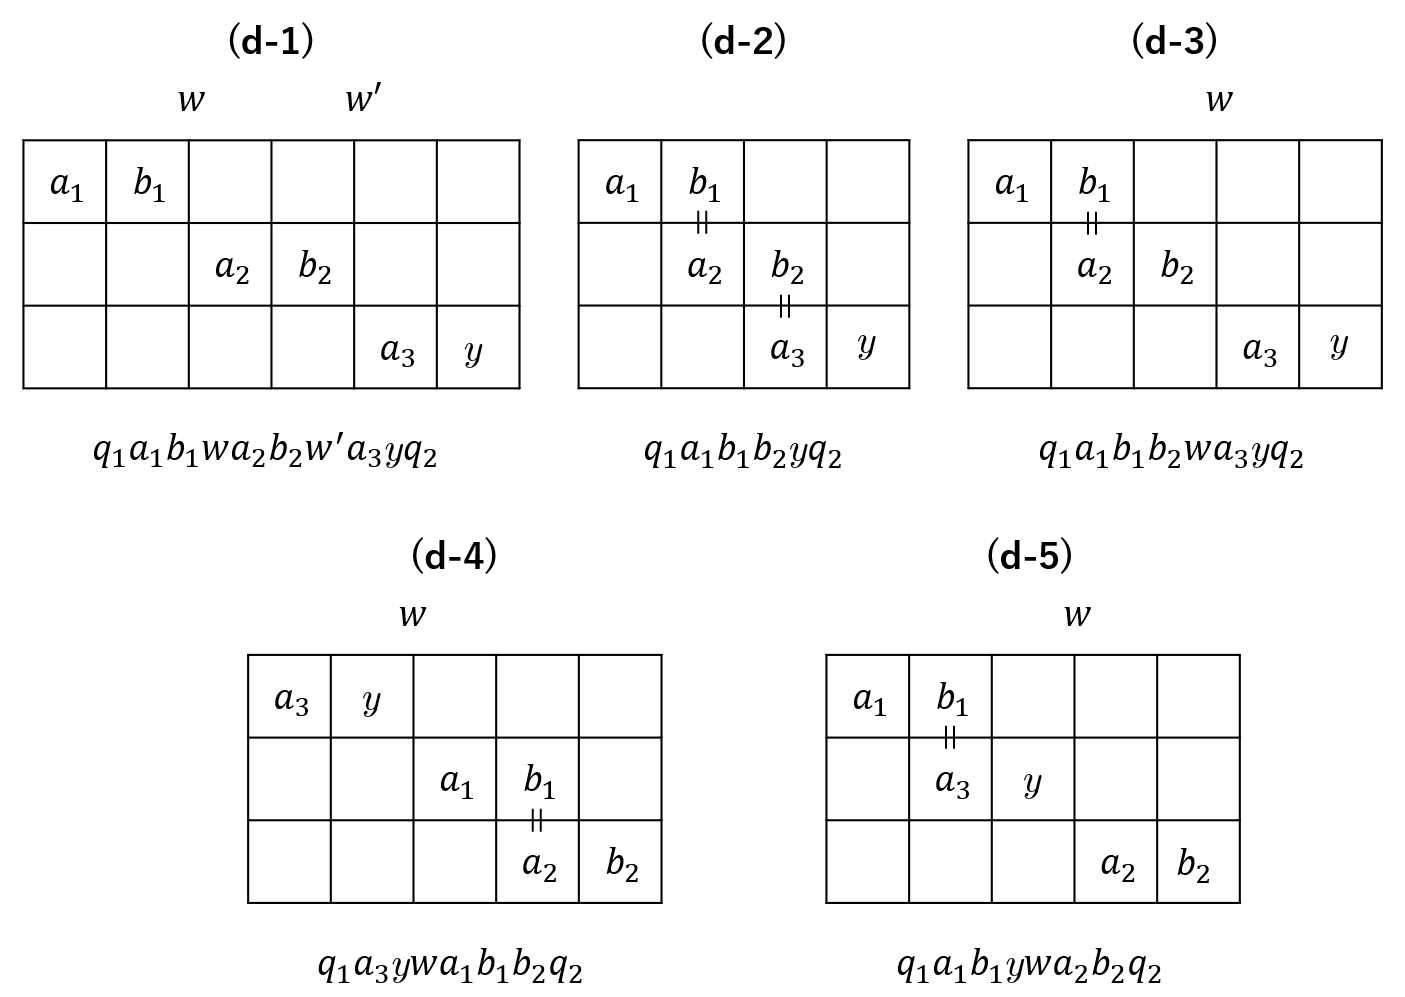
\includegraphics[width=\linewidth]{figs/Cases-d.png}
\vspace{-1cm}
\caption{(d)の場合分け}
\label{d組み合わせ}
\end{figure}

$C=a_{3}y$のとき,3つの記号列が重複する場合を考慮して,表\ref{d組み合わせ}のように,5つの場合に分けて証明する.
\[
\begin{tabular}{ll}
$\textbf{(d-1)}$ $q=q_{1}a_{1}b_{1}wa_{2}b_{2}w^{\prime}a_{3}yq_{2}$,\\
$\textbf{(d-2)}$ $q=q_{1}a_{1}b_{1}b_{2}yq_{2}$ ($a_{2}=b_{1}$かつ$a_{3}=b_{2}$),\\
$\textbf{(d-3)}$ $q=q_{1}a_{1}b_{1}b_{2}wa_{3}yq_{2}$ ($b_{1}=a_{2}$),\\
$\textbf{(d-4)}$ $q=q_{1}a_{3}ywa_{1}b_{1}b_{2}q_{2}$ ($b_{1}=a_{2}$),\\
$\textbf{(d-5)}$ $q=q_{1}a_{1}b_{1}ywa_{2}b_{2}q_{2}$ ($b_{1}=a_{3}$).
\end{tabular}
\]

\textbf{(d-1)} $q=q_{1}a_{1}b_{1}wa_{2}b_{2}w^{\prime}a_{3}yq_{2}$とする.これに対して,次の式が成り立っているものとする.
\begin{align*}
(1)~& p_{1} \preceq q_{1} & (\text{1'})~& p_{2} \preceq wa_{2}b_{2}w^{\prime}a_{3}yq_{2} \\
(2)~& p_{1} \preceq q_{1}a_{1}b_{1}w & (\text{2'})~& p_{2} \preceq w^{\prime}a_{3}yq_{2} \\
(3)~& p_{1} \preceq q_{1}a_{1}b_{1}wa_{2}b_{2}w^{\prime} & (\text{3'})~& p_{2} \preceq q_{2}
\end{align*}

$|w|+1=|w^{\prime}|$のとき,(2)と(3)より,$p_{1}$の接尾辞は$a_{1}b_{1}wa_{2}b_{2}w^{\prime}$かつ$a_{1}b_{1}w$である.
$w^{\prime}=w_{1}w$とおくと,$a_{1}b_{1}wa_{2}b_{2}w^{\prime}=a_{1}b_{1}wa_{2}b_{2}w_{1}w$と表すことができる.
$b_{2}w_{1}w=a_{1}b_{1}w$より,$b_{2}=a_{1}$となる.
(1')と(2')より,$p_{2}$の接頭辞は$wa_{2}b_{2}w^{\prime}a_{3}$かつ$w^{\prime}a_{3}$である.
$w^{\prime}=ww_{2}$とおくと, $w^{\prime}a_{3}=ww_{2}a_{3}$と表すことができる.$wa_{2}b_{2}=ww_{2}a_{3}$より,$b_{2}=a_{3}$となる.
よって,$b_{2}=a_{1}$より,$a_{1}=a_{3}$となり,$a_{1} \ne a_{3}$であることに矛盾する.

$|w|+1 < |w^{\prime}|$のとき,(2)と(3)より,$p_{1}$の接尾辞は$a_{1}b_{1}wa_{2}b_{2}w^{\prime}$かつ$a_{1}b_{1}w$である.
$w^{\prime}=w_{1}w$とおくと,$a_{1}b_{1}wa_{2}b_{2}w^{\prime}=a_{1}b_{1}wa_{2}b_{2}w_{1}w$と表すことができる.
よって,$w_{1}$の接尾辞は$a_{1}b_{1}$となる.
(1')と(2')より,$p_{2}$の接頭辞は$wa_{2}b_{2}w^{\prime}a_{3}$かつ$w^{\prime}a_{3}$である.
$w^{\prime}=w_{1}w$とおくと,$wa_{2}b_{2}w^{\prime}a_{3}=wa_{2}b_{2}w_{1}wa_{3}$となる.
さらに,$w^{\prime}=ww_{2}$とおくと,$w^{\prime}a_{3}=ww_{2}a_{3}$と表すことができる.$|a_{2}b_{2}w_{1}|=|w_{2}a_{3}|+1$より,$w_{1}$の最後から2つ目の記号は$a_{3}$となる.よって,$w_{1}$の接尾辞は$a_{1}b_{1}$であり,$a_{1}=a_{3}$となる.
これは,$a_{1} \ne a_{3}$であることに矛盾する.

$|w^{\prime}|+1=|w|$のとき,(1')と(2')より,$p_{2}$の接頭辞は$wa_{2}b_{2}w^{\prime}a_{3}$かつ$w^{\prime}a_{3}$である.
$w=w^{\prime}w_{1}$とおくと,$wa_{2}b_{2}w^{\prime}a_{3}=w^{\prime}w_{1}a_{2}b_{2}w^{\prime}a_{3}$と表すことができる.
$w^{\prime}w_{1}=w^{\prime}a_{3}$より,$w_{1}=a_{3}$となる.(2)と(3)より,$p_{1}$の接尾辞は$a_{1}b_{1}wa_{2}b_{2}w^{\prime}$かつ$a_{1}b_{1}w$である.
$w=w^{\prime}w_{1}$とおくと,$a_{1}b_{1}wa_{2}b_{2}w^{\prime}=a_{1}b_{1}w^{\prime}w_{1}a_{2}b_{2}w^{\prime}$となる.
さらに,$w=w_{2}w^{\prime}$とおくと,$a_{1}b_{1}w=a_{1}b_{1}w_{2}w^{\prime}$と表すことができる.
$|w_{1}a_{2}b_{2}w^{\prime}|=|a_{1}b_{1}w_{2}w^{\prime}|$より,$w_{1}=a_{1}$となる.よって,$w_{1}=a_{3}$より,$a_{1}=a_{3}$となり,$a_{1} \ne a_{3}$であることに矛盾する.

$|w| > |w^{\prime}|+1$のとき,(1')と(2')より,$p_{2}$の接頭辞は$wa_{2}b_{2}w^{\prime}a_{3}$かつ$w^{\prime}a_{3}$である.
$w=w^{\prime}w_{1}$とおくと,$wa_{2}b_{2}w^{\prime}a_{3}=w^{\prime}w_{1}a_{2}b_{2}w^{\prime}a_{3}$と表すことができる.
このとき,$w_{1}$の最初の記号は$a_{3}$となる.(2)と(3)より,$p_{1}$の接尾辞は$a_{1}b_{1}wa_{2}b_{2}w^{\prime}$かつ$a_{1}b_{1}w$である.
$w=w^{\prime}w_{1}$とおくと,$a_{1}b_{1}wa_{2}b_{2}w^{\prime}=a_{1}b_{1}w^{\prime}w_{1}a_{2}b_{2}w^{\prime}$となる.
さらに,$w=w_{2}w^{\prime}$とおくと,$a_{1}b_{1}w=a_{1}b_{1}w_{2}w^{\prime}$と表すことができる.
$|w_{1}a_{2}b_{2}|=|a_{1}b_{1}w_{2}|$より,$w_{1}$の接頭辞は$a_{1}b_{1}$となる.
よって,$w_{1}$の接頭辞は$a_{3}$であり,$a_{1}b_{1}$である.
すなわち,$a_{3}=a_{1}$となる.
これは,$a_{3} \ne a_{1}$であることに矛盾する.
\smallskip

\textbf{(d-2)} $q=q_{1}a_{1}b_{1}b_{2}yq_{2}$ ($a_{2}=b_{1}$かつ$a_{3}=b_{2}$)とする.
これに対して,次の式が成り立っているものとする.
\begin{align*}
(1)~& p_{1} \preceq q_{1} & (\text{1'})~& p_{2} \preceq b_{2}yq_{2} \\
(2)~& p_{1} \preceq q_{1}a_{1} & (\text{2'})~& p_{2} \preceq yq_{2} \\
(3)~& p_{1} \preceq q_{1}a_{1}b_{1} & (\text{3'})~& p_{2} \preceq q_{2}
\end{align*}

(2)と(3)より,$p_{1}$の接尾辞は$a_{1}b_{1}$かつ$a_{1}$である.
よって,$b_{1}=a_{1}$となる.$a_{2}=b_{1}$より,$a_{1}=a_{2}$となり,$a_{1} \ne a_{2}$であることに矛盾する.
\smallskip

\textbf{(d-3)} $q=q_{1}a_{1}b_{1}b_{2}wa_{3}yq_{2}$ ($b_{1}=a_{2}$)とする.これに対して,次の式が成り立っているものとする.
\begin{align*}
(1)~& p_{1} \preceq q_{1} & (\text{1'})~& p_{2} \preceq b_{2}wa_{3}yq_{2} \\
(2)~& p_{1} \preceq q_{1}a_{1} & (\text{2'})~& p_{2} \preceq wa_{3}yq_{2} \\
(3)~& p_{1} \preceq q_{1}a_{1}b_{1}b_{2}w & (\text{3'})~& p_{2} \preceq q_{2}
\end{align*}

$w=\varepsilon$のとき,(2)と(3)より,$p_{1}$の接尾辞は$a_{1}$かつ$a_{1}b_{1}b_{2}$である.
よって,$a_{1}=b_{2}$となる.
(1')と(2')より,$p_{2}$の接頭辞は$b_{2}a_{3}$かつ$a_{3}$である.
よって,$b_{2}=a_{3}$となる.
したがって,$a_{1}=b_{2}$より,$a_{1}=a_{3}$となり,$a_{1} \ne a_{3}$であることに矛盾する.

$|w| \ge 1$のとき,(2)と(3)より,$p_{1}$の接尾辞は$a_{1}$かつ$a_{1}b_{1}b_{2}w$である.
よって,$w$の最後の記号は$a_{1}$となる.
(1')と(2')より,$p_{2}$の接頭辞は$b_{2}wa_{3}$かつ$wa_{3}$である.
よって,$w$の最後の記号は$a_{3}$となる.
したがって,$w$の最後の記号は$a_{1}=a_{3}$となり,$a_{1} \ne a_{3}$であることに矛盾する.
\smallskip

\textbf{(d-4)} $q=q_{1}a_{3}ywa_{1}b_{1}b_{2}q_{2}$ ($b_{1}=a_{2}$)とする.これに対して,次の式が成り立っているものとする.
\begin{align*}
(1)~& p_{1} \preceq q_{1} & (\text{1'})~& p_{2} \preceq wa_{1}b_{1}b_{2}q_{2} \\
(2)~& p_{1} \preceq q_{1}a_{3}yw & (\text{2'})~& p_{2} \preceq b_{2}q_{2} \\
(3)~& p_{1} \preceq q_{1}a_{3}ywa_{1} & (\text{3'})~& p_{2} \preceq q_{2}
\end{align*}

(3)より,正規パターン$p_{1}^{\prime}$と$p_{1}^{\prime\prime}$が存在して,$p_{1}=p_{1}^{\prime}p_{1}^{\prime\prime}$,$p_{1}^{\prime} \preceq q_{1}a_{3}$かつ$p_{1}^{\prime\prime} \preceq ywa_{1}$が成り立つ.
これらより,$p=p_{1}xp_{2}=p_{1}^{\prime}p_{1}^{\prime\prime}xp_{2}\preceq q_{1}a_{3}p_{1}^{\prime\prime}xwa_{1}b_{1}b_{2}q_{2}=q \{ y := p_{1}^{\prime\prime}x \}$となるので,$p \preceq q$となり,$p \{ x := xy \} \preceq q$である.これは仮定に矛盾する.
\smallskip

\textbf{(d-5)} $q=q_{1}a_{1}b_{1}ywa_{2}b_{2}q_{2}$ ($b_{1}=a_{3}$)とする.これに対して,次の式が成り立っているものとする.
\begin{align*}
(1)~& p_{1} \preceq q_{1} & (\text{1'})~& p_{2} \preceq ywa_{2}b_{2}q_{2} \\
(2)~& p_{1} \preceq q_{1}a_{1} & (\text{2'})~& p_{2} \preceq wa_{2}b_{2}q_{2} \\
(3)~& p_{1} \preceq q_{1}a_{1}b_{1}yw & (\text{3'})~& p_{2} \preceq q_{2}
\end{align*}

$q_{1}^{\prime}=q_{1}a_{1}b_{1}$,$q_{2}^{\prime}=yw$,$q_{3}^{\prime}=a_{2}b_{2}q_{2}$とおくと,(3)から,$p_{1} \preceq q_{1}^{\prime}q_{2}^{\prime}$,(1')から$p_{2} \preceq q_{2}^{\prime}q_{3}^{\prime}$が得られ,さらに$q_{2}^{\prime}$は変数記号が含まれるので,補題\ref{補題9}より,$p \preceq q$となり,$p \{ x := xy \} \preceq q$である.
これは仮定に矛盾する.
%\hspace{\fill}\rm{(Q.E.D)}

\end{proof}

\begin{lem}\label{追加部分}
$\sharp \Sigma \ge 3$とし,$p, q$を正規パターンとする.
正規パターンの有限集合$D= \{ ya, bc, dy \}$ $(b \not = a,d$ かつ $c \not = a,d)$で表されるとき,任意の$r \in D$に対して$p \{ x := r \} \preceq q$ならば,$p \{ x := xy \} \preceq q$である.
\end{lem}
\begin{proof}
$p$に変数記号が現れない場合は自明である.
したがって,$p=p_{1}xp_{2}$ ($p_{1}, p_{2}$は正規パターン,$x$は変数記号)とおく.$p \{ x := xy \} \not \preceq q$と仮定して,矛盾を導く.

記号列$A,B,C$に対して,$\{ A,B,C \} = \{ y_{1}a,bc,dy_{2} \}$とおき,$q=q_{1}AwBw^{\prime}Cq_{2}$とする.
これに対して,次の式が成り立っているものとする.
\begin{align*}
(1)~& p_{1} \preceq q_{1} & (\text{1'})~& p_{2} \preceq wBw^{\prime}Cq_{2} \\
(2)~& p_{1} \preceq q_{1}Aw & (\text{2'})~& p_{2} \preceq w^{\prime}Cq_{2} \\
(3)~& p_{1} \preceq q_{1}AwBw^{\prime} & (\text{3'})~& p_{2} \preceq q_{2}
\end{align*}

$q^{\prime}_{1}=q_{1}A,~q^{\prime}_{2}=wBw^{\prime},~q^{\prime}_{3}=Cq_{2}$とおくと,(3)と(1')より,$p_{1} \preceq q^{\prime}_{1}q^{\prime}_{2},~p_{2} \preceq q^{\prime}_{2}q^{\prime}_{3}$となる.
補題\ref{補題9}より,$q^{\prime}_{2}$に変数記号が含まれるとき,$p \preceq q$となる.
よって,$B=y_{1}a$または,$B=dy_{2}$である場合,仮定に矛盾する.
したがって,$B=bc$である場合のみを考える.

$A=dy_{2}$とすると,(2)は$p_{1} \preceq q_{1}dy_{2}w$となる.
$p_{1}=p^{\prime}_{1}p^{\prime\prime}_{1}, p^{\prime}_{1} \preceq q_{1}d$かつ$p^{\prime\prime}_{1} \preceq y_{2}w$とおくと,(1')より,$p=p_{1}xp_{2}=p^{\prime}_{1}p^{\prime\prime}_{1}xp_{2} \preceq q_{1}dp^{\prime\prime}_{1}xwbcw^{\prime}y_{1}aq_{2}=q \{ x:=p^{\prime\prime}_{1}x \}$となり,$p=q\theta$となる.
これは仮定に矛盾する.
したがって,$A=y_{1}a,B=bc,C=dy_{2}$である場合のみ考えればよい.

$q=q_{1}y_{1}awbcw^{\prime}dy_{2}q_{2}~(b \not = a,d$かつ$c \not = a,d)$とする.
これに対して,次の式が成り立っているものとする.
\begin{align*}
(1)~& p_{1} \preceq q_{1} & (\text{1'})~& p_{2} \preceq wbcw^{\prime}dy_{2}q_{2} \\
(2)~& p_{1} \preceq q_{1}y_{1}aw & (\text{2'})~& p_{2} \preceq w^{\prime}dy_{2}q_{2} \\
(3)~& p_{1} \preceq q_{1}y_{1}awbcw^{\prime} & (\text{3'})~& p_{2} \preceq q_{2}
\end{align*}

$|w|=|w^{\prime}|$のとき,(2)と(3)より,$p_{1}$の接尾辞は$awbcw^{\prime}$かつ$aw$であるので,$cw^{\prime}=aw$となる.
これは,$c=a$となり,$c \not = a$であることに矛盾する.

$|w| = |w^{\prime}|+1$のとき,(2)と(3)より,$p_{1}$の接尾辞は$awbcw^{\prime}$かつ$aw$である.
$w=w_{1}w^{\prime}$とおくと,$aw=aw_{1}w^{\prime}$となる.
したがって,$bcw^{\prime}=aw_{1}w^{\prime}$より,$b = a$となる.
これは$b \not = a$であることに矛盾する.

$|w| = |w^{\prime}|+2$のとき,(2)と(3)より,$p_{1}$の接尾辞は$awbcw^{\prime}$かつ$aw$であり,(1')と(2')より,$p_{2}$の接頭辞は$wbcw^{\prime}d$かつ$w^{\prime}d$である.

%\begin{figure}[H]
\begin{figure}  
\centering
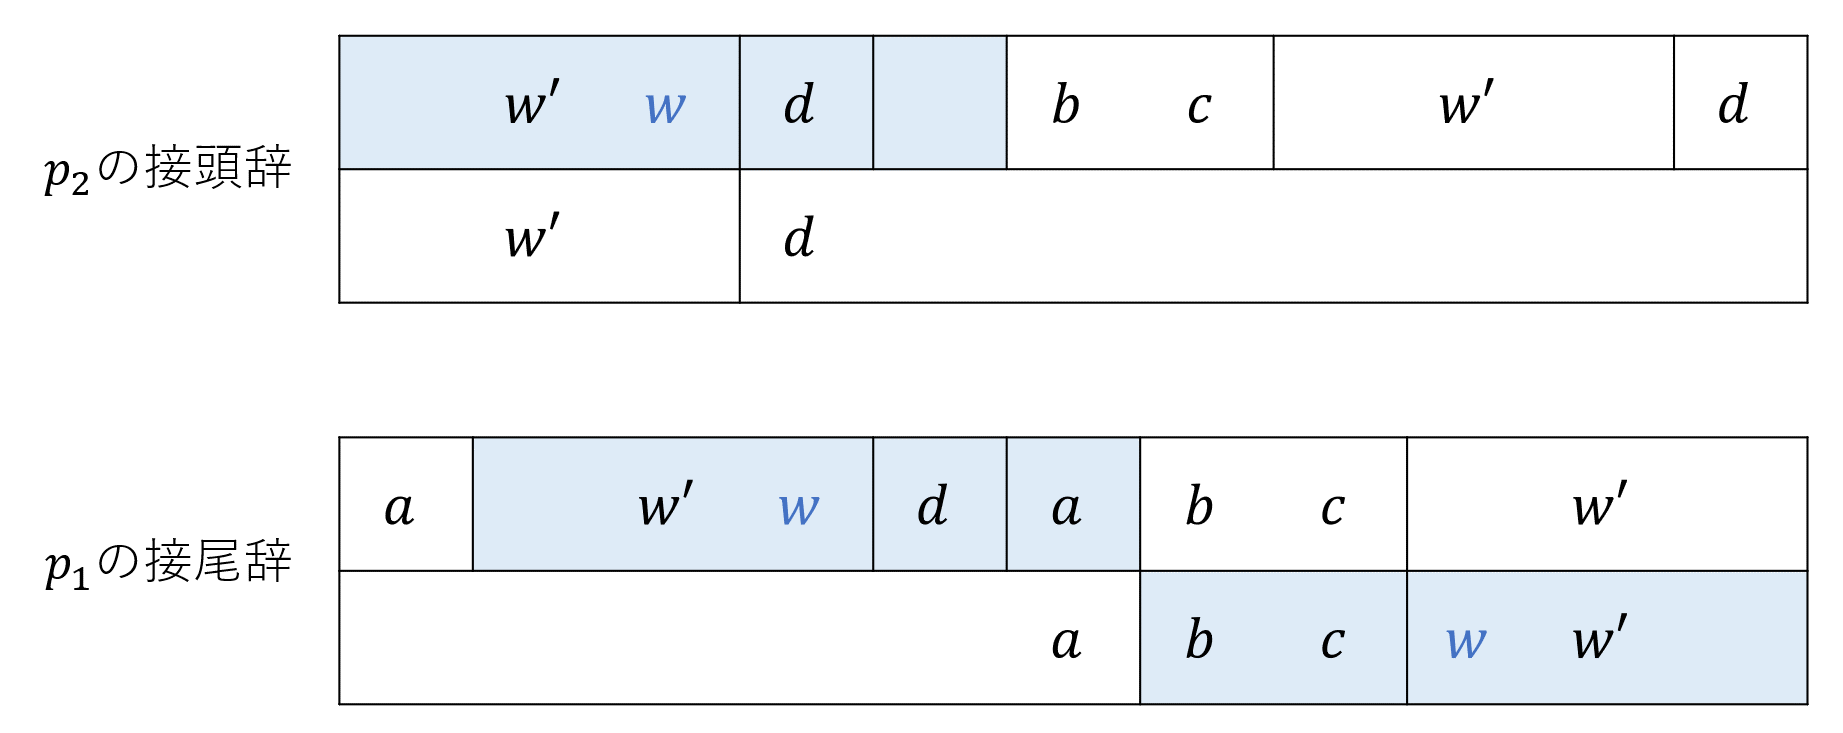
\includegraphics[width=\linewidth]{figs/Pre-Suff.png}
\vspace{-1cm}
\caption{$|w| = |w^{\prime}|+2$における\,$p_{1}$\,の接尾辞,$p_{2}$\,の接頭辞の関係}
\label{追加部分1}
\vspace*{-.2cm}
\end{figure}

図\ref{追加部分1}のように,$w=w^{\prime}da,~w=bcw^{\prime}$となる.
よって,$w^{\prime}da=bcw^{\prime}$となる.

\begin{cl}\label{主張1}
$w^{\prime}$を定数記号列,a,b,c,dを定数記号とする.
このとき,$w^{\prime}da \not =bcw^{\prime}$ $(b \not = a,d$かつ$c \not = a,d)$となる.
\end{cl}

\noindent\textbf{主張\ref{主張1}の証明.}
$w^{\prime}da=bcw^{\prime}$と仮定する.
$|w^{\prime}| \ge 4$のとき,$w^{\prime}=bcw_{1}da$ $(w_{1}$は定数記号列$)$とおける.
$w^{\prime}da=bcw_{1}dada, bcw^{\prime}=bcbcw_{1}da$であるので,$bcw_{1}dada=bcbcw_{1}da$となる.
$w^{\prime}$と同様に$w_{1}$を考えると,$w_{1}=bcw_{2}da$ $(w_{2}$は定数記号列$)$とおける.
$w_{2}$以降も同様に定義できる.
ここで,定数記号列の長さを考えていくと,$|w_{1}|=|w^{\prime}|-4, |w_{2}|=|w_{1}|-4$のように,$|w_{i+1}|$は$|w_{i}|$より長さ4ずつ短くなっていく.
そのため,定数記号列を繰り返し定義していくと,最終的に定義できる$w_{n}$は長さ0,1,2,3のいずれかとなる.

%\begin{figure}[H]
\begin{figure}  
\centering
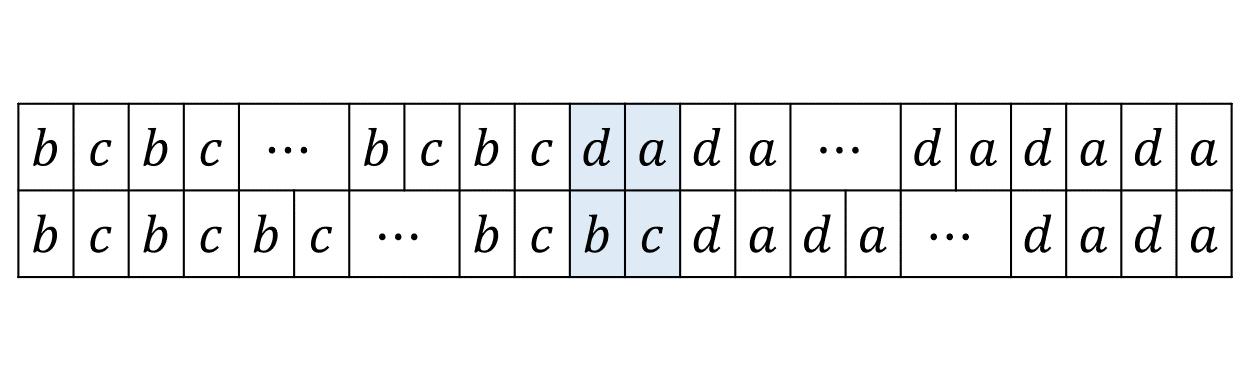
\includegraphics[width=\linewidth]{figs/ConstantSeq.png}
\vspace{-1.5cm}
\caption{$|w_{n}| = 0$における定数記号列}
\label{追加部分2}
\vspace*{-.2cm}
\end{figure}


$|w_{n}|=0$のとき,図\ref{追加部分2}のように,$da=bc$となる.
これは,$b \not = d$であることに矛盾する.

%\begin{figure}[H]
\begin{figure}
\centering
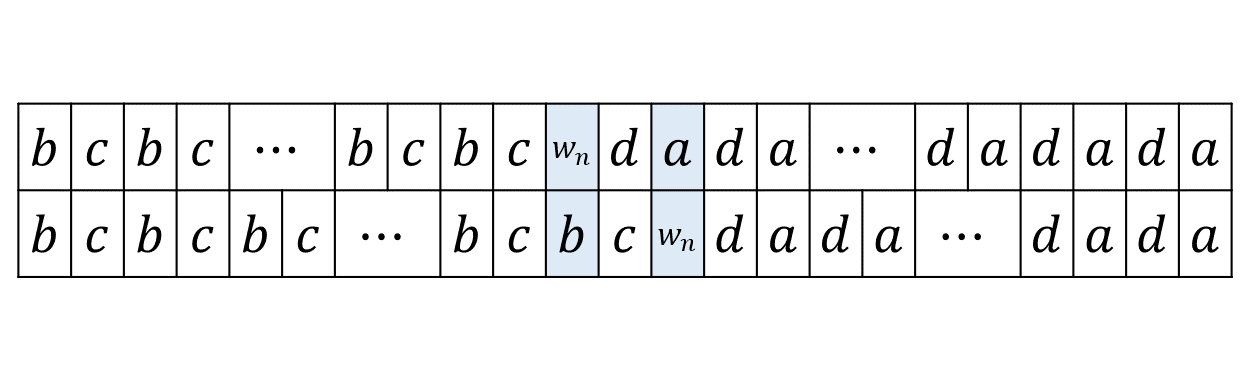
\includegraphics[width=\linewidth]{figs/w_n=1.png}
\vspace{-1.5cm}
\caption{$|w_{n}| = 1$における定数記号列}
\label{追加部分3}
\vspace*{-.2cm}
\end{figure}


$|w_{n}|=1$のとき,図\ref{追加部分3}のように,$w_{n}=a=b$となる.
これは,$b \not = a$であることに矛盾する.

%\begin{figure}[H]
\begin{figure}  
\centering
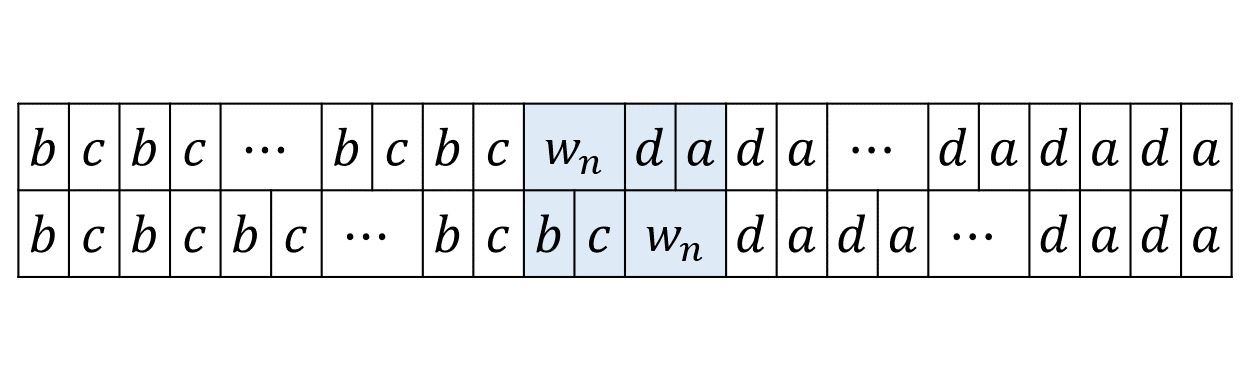
\includegraphics[width=\linewidth]{figs/w_n=2.png}
\vspace{-1.5cm}
\caption{$|w_{n}| = 2$における定数記号列}
\label{追加部分4}
\vspace*{-.2cm}
\end{figure}

$|w_{n}|=2$のとき,図\ref{追加部分4}のように,$w_{n}=bc=da$となる.
これは,$b \not = d$であることに矛盾する.

%\begin{figure}[H]
\begin{figure}  
\centering
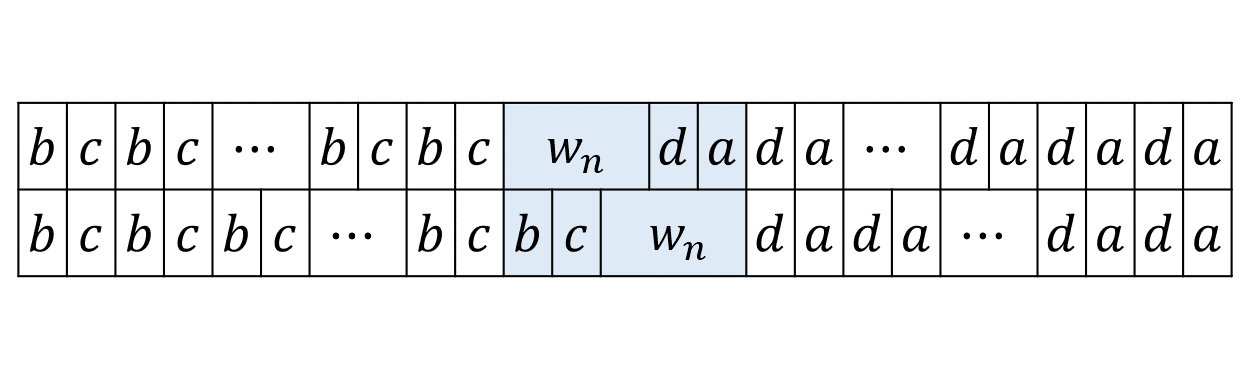
\includegraphics[width=\linewidth]{figs/w_n=3.png}
\vspace{-1.5cm}
\caption{$|w_{n}| = 3$における定数記号列}
\label{追加部分5}
\end{figure}

$|w_{n}|=3$のとき,$w_{n}=w_{n_{1}}w_{n_{2}}w_{n_{3}} (w_{n_{i}}$は$w_{n}$におけるi番目の定数記号$)$と表すと,図\ref{追加部分5}のように,$bcw_{n_{3}}=w_{n_{1}}da$となる.
よって,$c=d$となる.
これは,$c \not = d$であることに矛盾する.

以上より,$|w_{n}|=0,1,2,3$のとき,すべての場合において,仮定に矛盾するため,$|w^{\prime}| \ge 4$である場合,$w^{\prime}da \not = bcw^{\prime}$となる.

$|w^{\prime}| \le 3$のとき,$|w_{n}|=0,1,2,3$を$|w^{\prime}|$と置き換えて考えることができるため,すべての場合において仮定に矛盾する.
よって,$w^{\prime}da \not = bcw^{\prime}$となる.

\hspace{\fill}\rm{(主張\ref{主張1}のQ.E.D)}

よって,$w^{\prime}da=bcw^{\prime}$は,主張\ref{主張1}に矛盾する.

%\begin{figure}[H]
\begin{figure}  
\centering
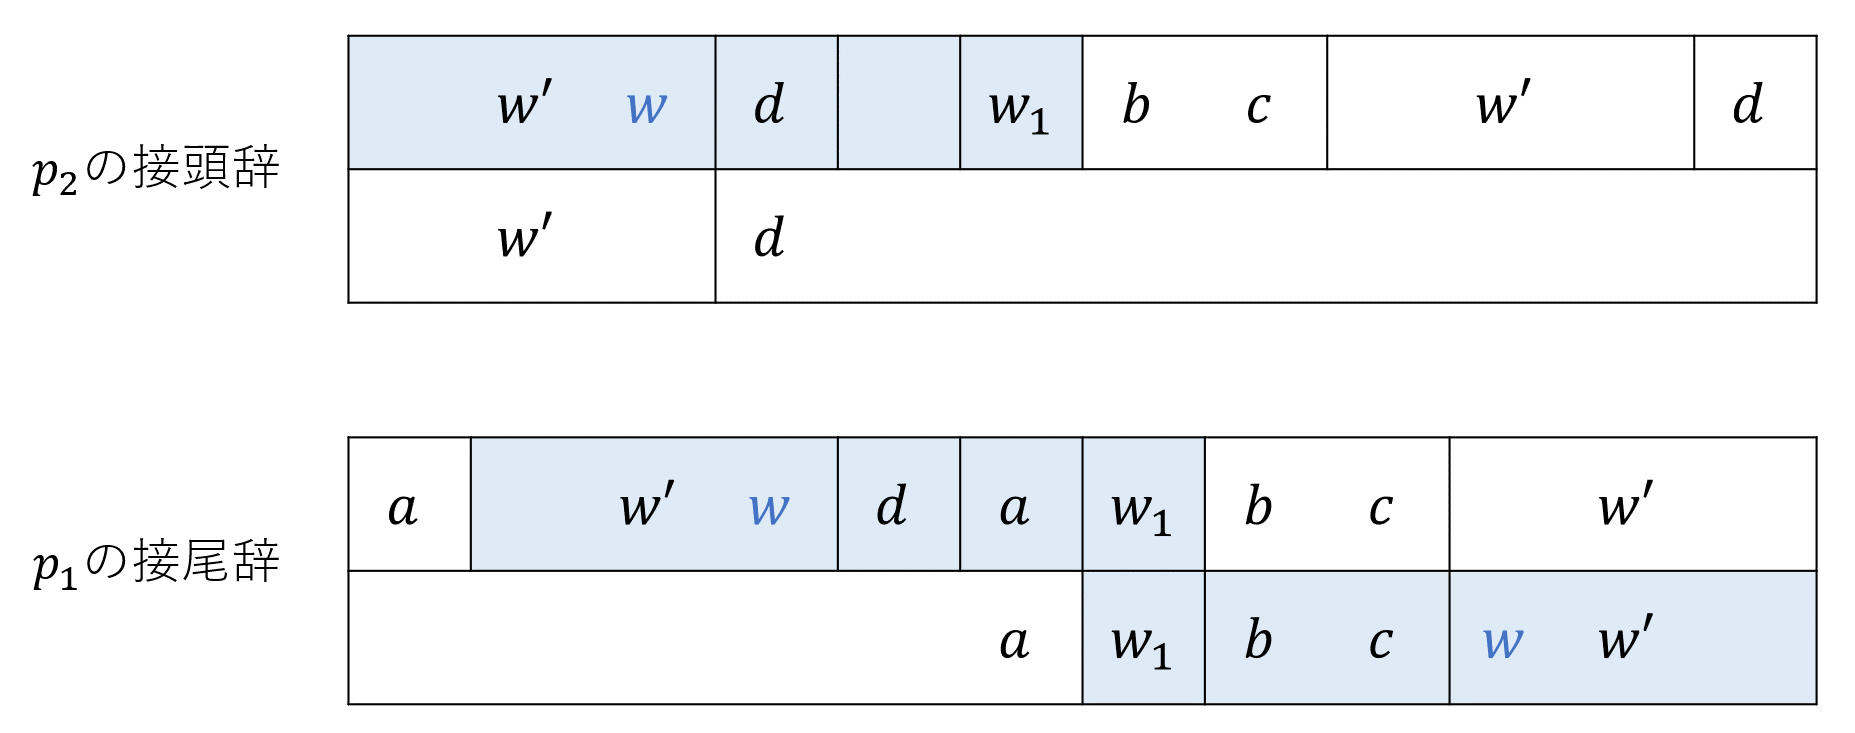
\includegraphics[width=\linewidth]{figs/wgewprime+3.png}
\vspace{-1cm}
\caption{$|w| \ge |w^{\prime}|+3$における$p_{1}$の接尾辞,$p_{2}$の接頭辞の関係}
\label{追加部分6}
\end{figure}

$|w| \ge |w^{\prime}|+3$のとき,図\ref{追加部分6}のように,$w=w^{\prime}daw_{1}=w_{1}bcw^{\prime}$ $(w_{1}$は定数記号列$)$となる.
よって,$w^{\prime}daw_{1}=w_{1}bcw^{\prime}$となる.

\begin{cl}\label{主張2}
$w, w_{1}$を定数記号列,a,b,c,dを定数記号とする.
このとき,$wdaw_{1} \not =w_{1}bcw$ $(b \not = a,d$かつ$c \not = a,d)$となる.
\end{cl}

\noindent\textbf{主張\ref{主張2}の証明.}
$wdaw_{1}=w_{1}bcw$と仮定する.
$w$と$w_{1}$の関係を以下のように場合分けして,考えていく.
\[
\begin{tabular}{ll}
$\textbf{(a)}$ $|w_{1}| \le |w| \le |w_{1}|+2$,\\
$\textbf{(b)}$ $2|w_{1}| \le |w| \le 2|w_{1}|+4$,\\
$\textbf{(c)}$ $|w_{1}|=0$,\\
$\textbf{(d)}$ $|w_{1}|+3 \le |w| \le 2|w_{1}|-1$,\\
$\textbf{(e)}$ $|w| \ge 2|w_{1}|+5$. 
\end{tabular}
\]

\noindent$\textbf{(a)}$ $|w_{1}| \le |w| \le |w_{1}|+2$である場合から考える.

%\begin{figure}[H]
\begin{figure} 
\centering
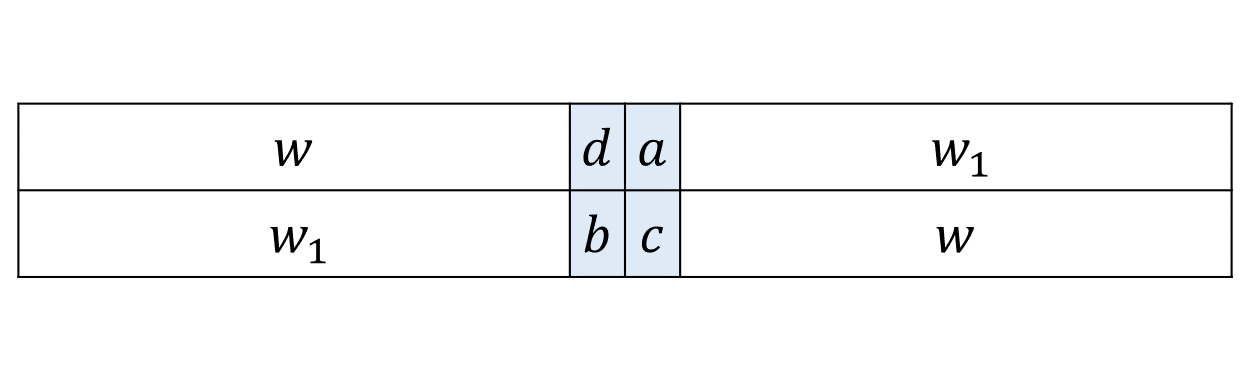
\includegraphics[width=\linewidth]{figs/w=w_1.png}
\vspace{-1.5cm}
\caption{$|w| = |w_{1}|$における定数記号列}
\label{追加部分7}
\vspace*{-.4cm}
\end{figure}

$|w|=|w_{1}|$のとき,図\ref{追加部分7}のように,$bc=da$となる.
これは,$b \not = d$であることに矛盾する.

%\begin{figure}[H]
\begin{figure}  
\centering
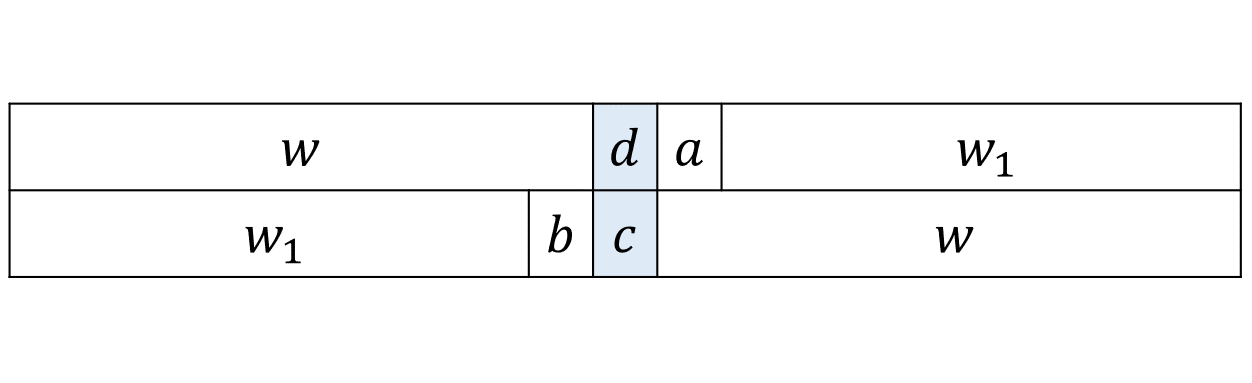
\includegraphics[width=\linewidth]{figs/w=w_1+1.png}
\vspace{-1.5cm}
\caption{$|w| = |w_{1}|+1$における定数記号列}
\label{追加部分8}
\vspace*{-.4cm}
\end{figure}

$|w|=|w_{1}|+1$のとき,図\ref{追加部分8}のように,$c=d$となる.
これは,$c \not = d$であることに矛盾する.

%\begin{figure}[H]
%\begin{figure}  
%\centering
%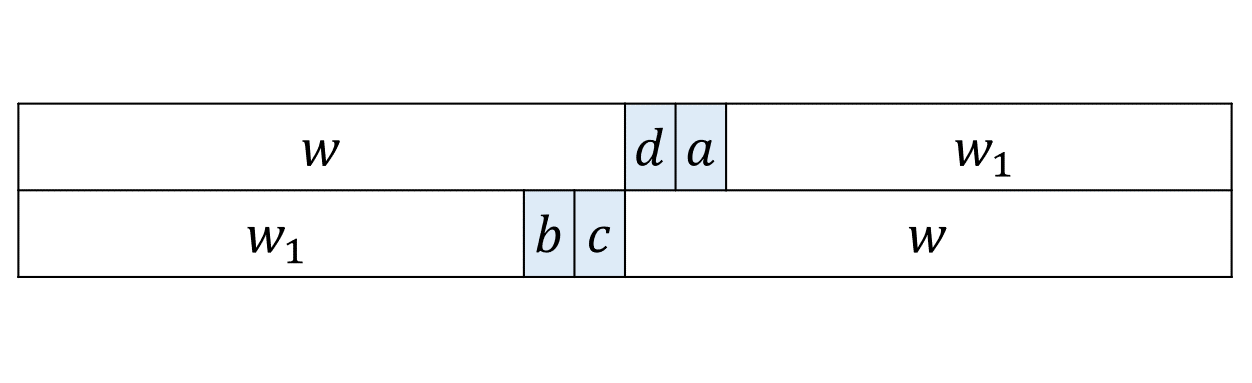
\includegraphics[width=\linewidth]{figs/追加部分9.png}
%\vspace{-1.5cm}
%\caption{$|w| = |w_{1}|+2$における定数記号列}
%\label{追加部分9}
%\vspace*{-.4cm}
%\end{figure}

$|w|=|w_{1}|+2$のとき,図\ref{追加部分9}のように,$w=w_{1}bc=daw_{1}$となる.
これは,主張\ref{主張1}に矛盾する.

\noindent$\textbf{(b)}$ $2|w_{1}| \le |w| \le 2|w_{1}|+4$である場合,

$|w|=2|w_{1}|$のとき,図\ref{追加部分14}のように,$w_{1}da=bcw_{1}$となる.
これは,主張\ref{主張1}に矛盾する.

$|w|=2|w_{1}|+1$のとき,図\ref{追加部分13}のように,$b=a$となる.
これは,$b \not = a$であることに矛盾する.

$|w|=2|w_{1}|+2$のとき,図\ref{追加部分12}のように,$bc=da$となる.
これは,$b \not = d$であることに矛盾する.

$|w|=2|w_{1}|+3$のとき,図\ref{追加部分11}のように,$c=d$となる.
これは,$c \not = d$であることに矛盾する.

%\begin{figure}[H]
\begin{figure}  
\centering
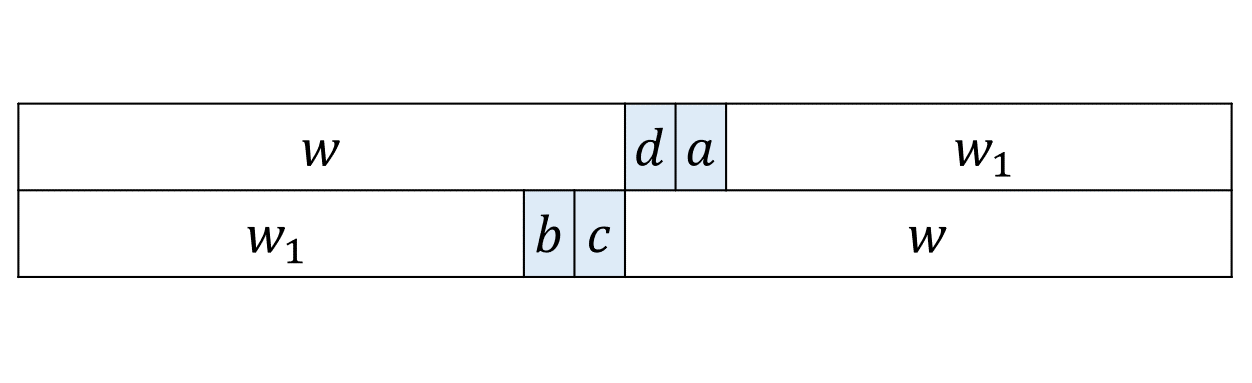
\includegraphics[width=\linewidth]{figs/w=w_1+2.png}
\vspace{-1.0cm}
\caption{$|w| = |w_{1}|+2$における定数記号列}
\label{追加部分9}
\vspace*{.5cm}

\centering
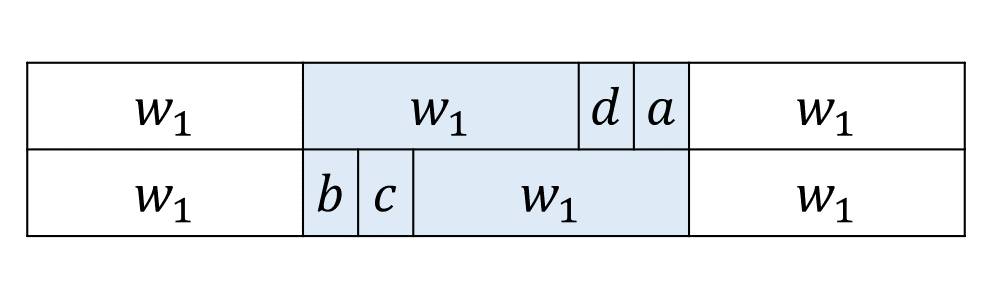
\includegraphics[scale=.4]{figs/w=2w_1.png}
\vspace{-.4cm}
\caption{$|w| = 2|w_{1}|$における定数記号列}
\label{追加部分14}
\vspace*{.5cm}
%\vspace*{-.2cm}
%\end{figure}
%
%\begin{figure}[H]
%\begin{figure}  
\centering
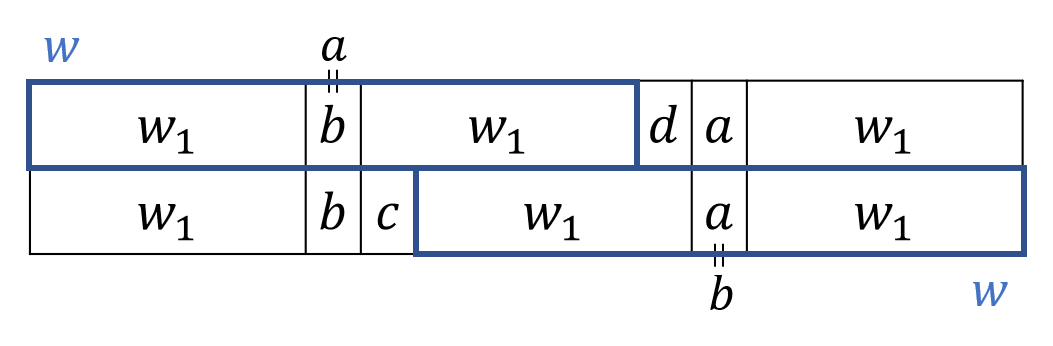
\includegraphics[scale=.4]{figs/w=2w_1+1.png}
\vspace{-.4cm}
\caption{$|w| = 2|w_{1}|+1$における定数記号列}
\label{追加部分13}
\vspace*{.5cm}
%\vspace*{-.4cm}
%\end{figure}
%
%
%\begin{figure}[H]
%\begin{figure}
\centering
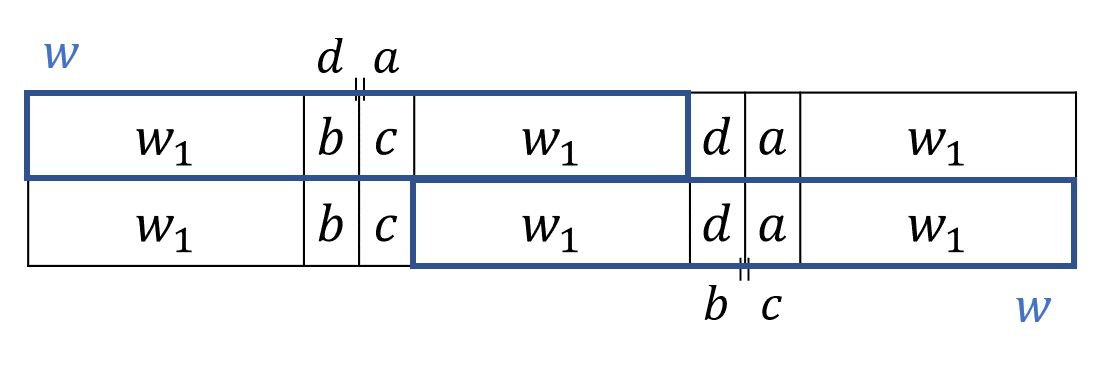
\includegraphics[scale=.4]{figs/w=2w_1+2.png}
\vspace{-.5cm}
\caption{$|w| = 2|w_{1}|+2$における定数記号列}
\label{追加部分12}
\vspace*{.5cm}
%\vspace*{-.4cm}
%\end{figure}
%
%
%\begin{figure}[H]
%\begin{figure} 
\centering
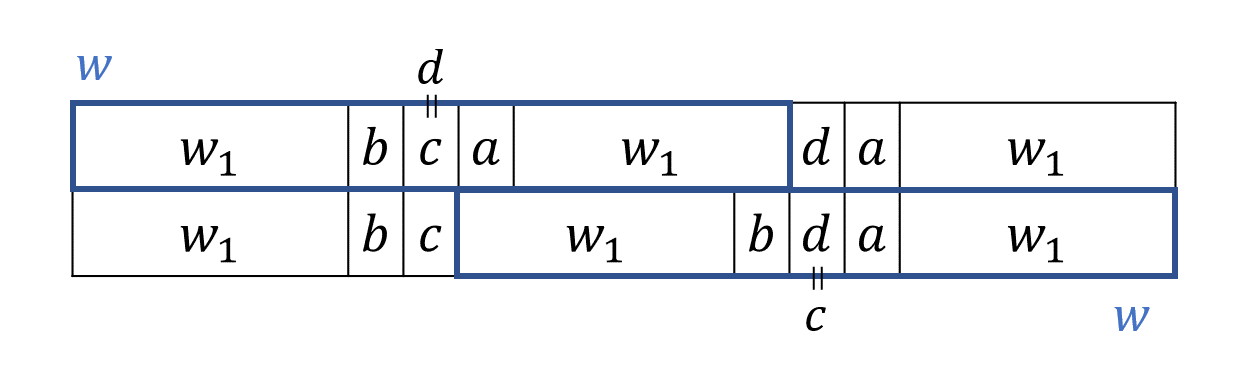
\includegraphics[width=\linewidth]{figs/w=2w_1+3.png}
\vspace{-1cm}
\caption{$|w| = 2|w_{1}|+3$における定数記号列}
\label{追加部分11}
\vspace*{.5cm}
%\vspace*{-.7cm}
%\end{figure}
%
%
%\begin{figure}[H]
%\begin{figure}
\centering
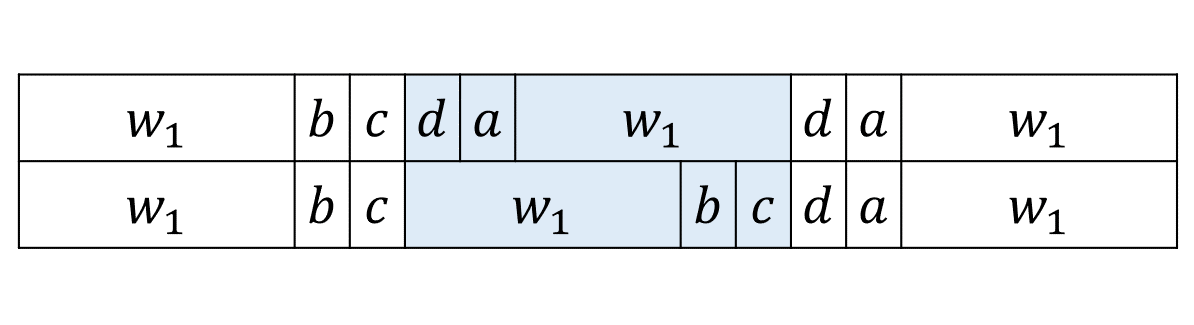
\includegraphics[width=\linewidth]{figs/w=2w_1+4.png}
\vspace{-1.2cm}
\caption{$|w| = 2|w_{1}|+4$における定数記号列}
\label{追加部分10}
%\vspace*{-.5cm}

%\centering
%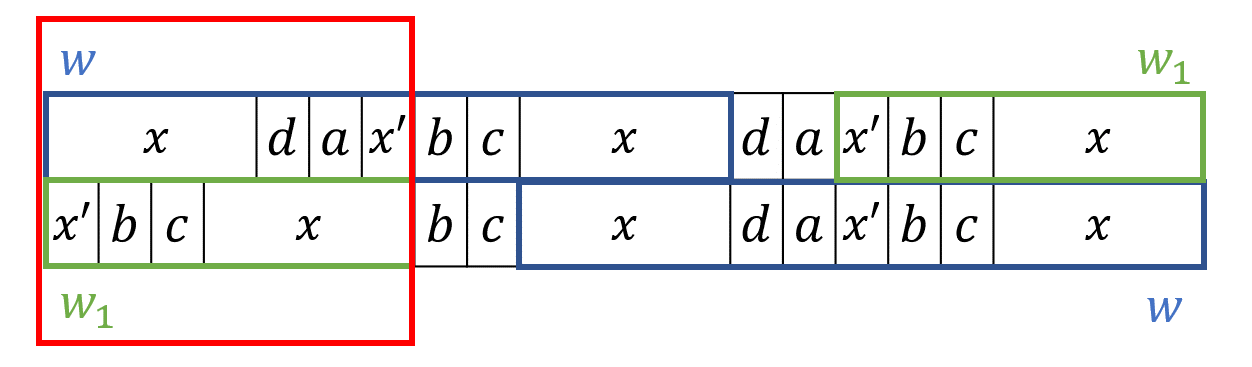
\includegraphics[width=\linewidth]{figs/w1+3.png}
%\vspace{-1cm}
%\caption{$|w_{1}|+3 \le |w| \le 2|w_{1}|-1$における定数記号列}
%\label{w1+3}
\end{figure}

$|w|=2|w_{1}|+4$のとき,$w=w_{1}bcdaw_{1}$とおける.
図\ref{追加部分10}のように,$daw_{1}=w_{1}bc$となる.
これは,主張\ref{主張1}に矛盾する.

\noindent$\textbf{(c)}$ $|w_{1}|=0$のとき,$wda \not = bcw$ $(b \not = a,d$かつ$c \not = a,d)$となる.
これは,主張\ref{主張1}に矛盾する.

上記以外の範囲$\textbf{(d)}$ $|w_{1}|+3 \le |w| \le 2|w_{1}|-1$と$\textbf{(e)}$ $|w| \ge 2|w_{1}|+5$である場合,対象とする定数記号列の長さを減らして考えることができる.

\noindent$\textbf{(d)}$ $|w_{1}|+3 \le |w| \le 2|w_{1}|-1$のとき,

%\begin{figure}[H]
%\begin{figure}
%\centering
%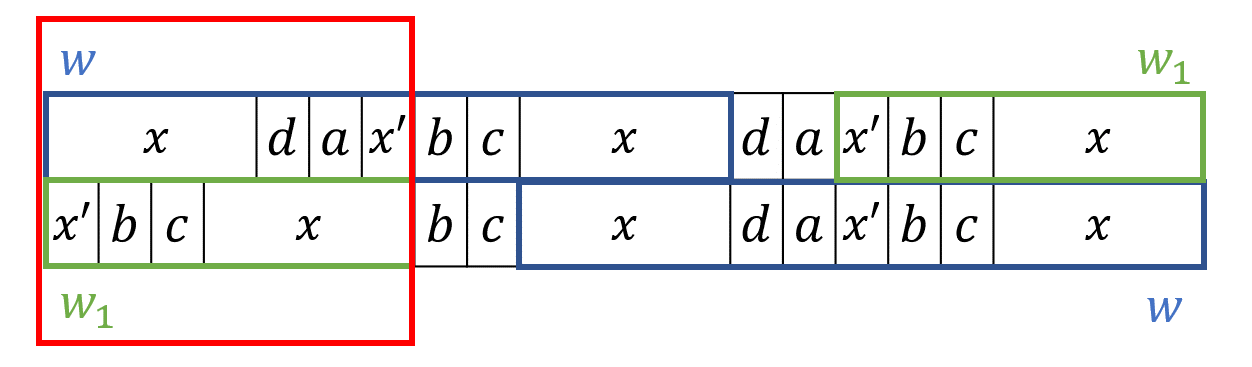
\includegraphics[width=\linewidth]{figs/w1+3.png}
%\vspace{-1cm}
%\caption{$|w_{1}|+3 \le |w| \le 2|w_{1}|-1$における定数記号列}
%\label{w1+3}
%\end{figure}

図\ref{w1+3}のように,$W$を$w$,$W^{\prime}$を$w_{1}$と置き換えて考えることができる.
よって,赤枠部分以外の定数記号列を無視できるため,対象とする定数記号列の長さを減らすことができる.

\noindent$\textbf{(e)}$ $|w| \ge 2|w_{1}|+5$のとき,

%\begin{figure}[H]
\begin{figure}
\centering
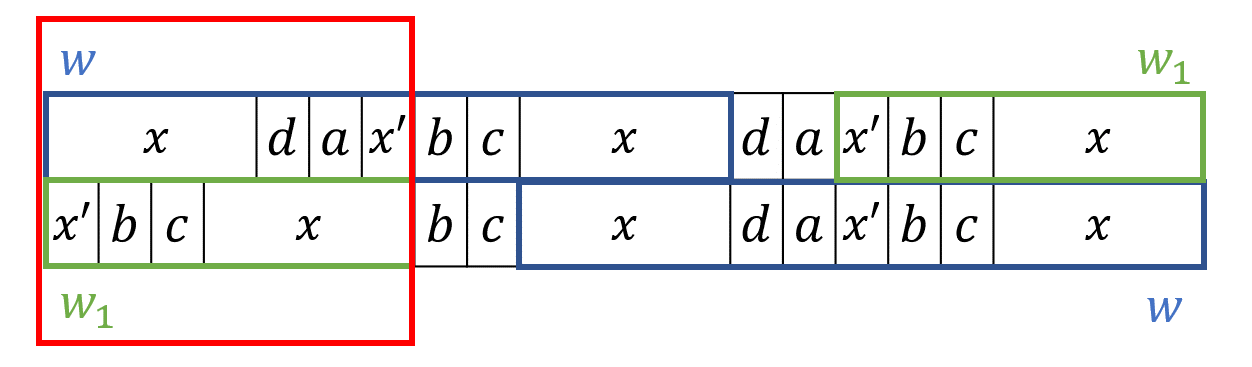
\includegraphics[width=\linewidth]{figs/w1+3.png}
\vspace{-1cm}
\caption{$|w_{1}|+3 \le |w| \le 2|w_{1}|-1$における定数記号列}
\label{w1+3}
%\vspace*{-.3cm}

\centering
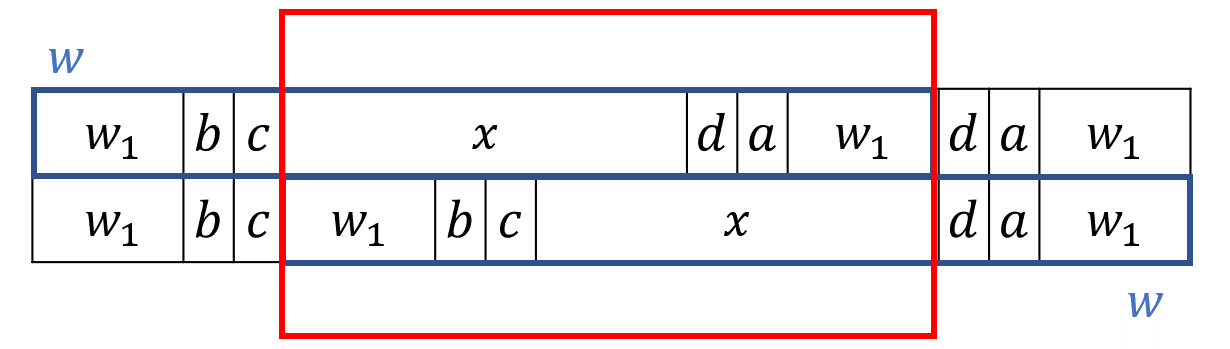
\includegraphics[width=\linewidth]{figs/2w1+5.png}
\vspace{-1cm}
\caption{$|w| \ge 2|w_{1}|+5$における定数記号列}
\label{2w1+5}
\vspace*{-.3cm}
\end{figure}

図\ref{2w1+5}のように,$W$と$w$を置き換えて考えることができる.
よって,赤枠部分以外の定数記号列を無視できるため,対象とする定数記号列の長さを減らすことができる.

したがって,$\textbf{(d)}$ $|w_{1}|+3 \le |w| \le 2|w_{1}|-1$と$\textbf{(e)}$ $|w| \ge 2|w_{1}|+5$の場合,$w,w_{1}$の長さを減らして考えることができる.
この結果より,$w$と$w_{1}$の長さの関係は,最終的に,$\textbf{(a)}$ $|w_{1}| \le |w| \le |w_{1}|+2$,$\textbf{(b)}$ $2|w_{1}| \le |w| \le 2|w_{1}|+4$,$\textbf{(c)}$ $|w_{1}|=0$のいずれかに当てはまるため,仮定に矛盾する.

\hspace{\fill}\rm{(主張\ref{主張2}のQ.E.D)}

よって,$w^{\prime}daw_{1}=w_{1}bcw^{\prime}$は,主張\ref{主張2}に矛盾する.
次に,$|w| < |w^{\prime}|$である場合を考える.

$|w^{\prime}|=|w|+1$のとき,(1')と(2')より,$p_{2}$の接頭辞は$wbcw^{\prime}d$かつ$w^{\prime}d$である.
$|wbc|=|w^{\prime}d|$より,$c=d$となる.
これは,$c \ne d$であることに矛盾する.

$|w^{\prime}|=|w|+2$のとき,(1')と(2')より,$p_{2}$の接頭辞は$wbcw^{\prime}d$かつ$w^{\prime}d$である.
$|wbc|=|w^{\prime}|$より,$w^{\prime}$の最初の記号は$d$となり,$w^{\prime}$の最後の2つの記号は$bc$となる.
(2)と(3)より,$p_{1}$の接尾辞は$awbcw^{\prime}$かつ$aw$であるため,$|w^{\prime}|-1=|aw|$より,$w^{\prime}$の最初から2つ目の記号は$a$となる.
よって,$w^{\prime}=wbc=daw$となる.
これは,主張\ref{主張1}に矛盾する.

$|w^{\prime}| \ge |w|+3$のとき,(1')と(2')より,$p_{2}$の接頭辞は$wbcw^{\prime}d$かつ$w^{\prime}d$である.
$|wbcw_{1}|=|w^{\prime}|$ ($w_{1}$は定数記号列)より,$w^{\prime}$の接頭辞は$w_{1}d$となり,$w^{\prime}$の接尾辞は$bcw_{1}$となる.
(2)と(3)より,$p_{1}$の接尾辞は$awbcw^{\prime}$かつ$aw$である.
$|w^{\prime}|-|w_{1}|-1=|aw|$より,$w^{\prime}$の最初から2つ目の記号は$a$となる.
よって,$w^{\prime}=wbcw_{1}=w_{1}daw$となる.
これは,主張\ref{主張2}に矛盾する.
\end{proof}

